\chapter{MULTILAYER DRIPPING HANDRAL}
\thispagestyle{empty}

\mquote{not selectet yet}{...}

The accretion disc model developed for this study is referred to as \emph{Multilayer Dripping Handrail} (MDH). The underlying hypothesis of our proposed model is that different physical systems will, in some aspects, behave very similarly (as we discussed in Chapter \ref{chap:similary_of_nonlinear_systems}). 

In our case, the demanding one is the magneto-hydrodynamical accretion disk system, which, if taken to the extreme, is composed of individual gas particles interacting. Such a model would be a direct solution of either plasma physics equations or Navier-Stokes equations with a magnetic field. It is clearly beyond the limits of today's hardware, or at least very complex. 

%%%%%%%%%%%%%
% The model %
%%%%%%%%%%%%%

\section{The model}

The MDH model takes inspiration from the model created by \cite{yonehara1997}, which uses a simple mass limit condition triggering the redistribution into lower adjacent cells. To take this concept further, we are implementing the Mass-Spring model (MSM) as a means of non-linear matter redistribution. We discussed the original MSM in detail in Chapter \ref{chap:dripping_faucet}. 

\subsection{The cellular accretion disk model}

Our MDH model is a cellular automaton constructed by arranging $I$ times $J$ individual cells in concentric rings (i.e., layers). The $I$ and $J$ values represent the grid dimensions. We denote the layers by 

\begin{equation}
i \in [0;I-1].
\end{equation}

The outermost layer is $i=0$. Each layer consists of $J$ individual cells denoted by

\begin{equation}
j \in [0;J-1].
\end{equation}

The direction in which we iterate over $j$ is arbitrary and is a matter of perspective. Because the layers orbit the imagined central object at differing angular velocities, the simulation grid naturally shifts over time. Figure \ref{fig:grid_states} shows possible simulation grid states. On the left is the initial simulation grid state, and on the right is the shifted state after an arbitrary number of simulation steps.

\begin{figure}[H]
\centering
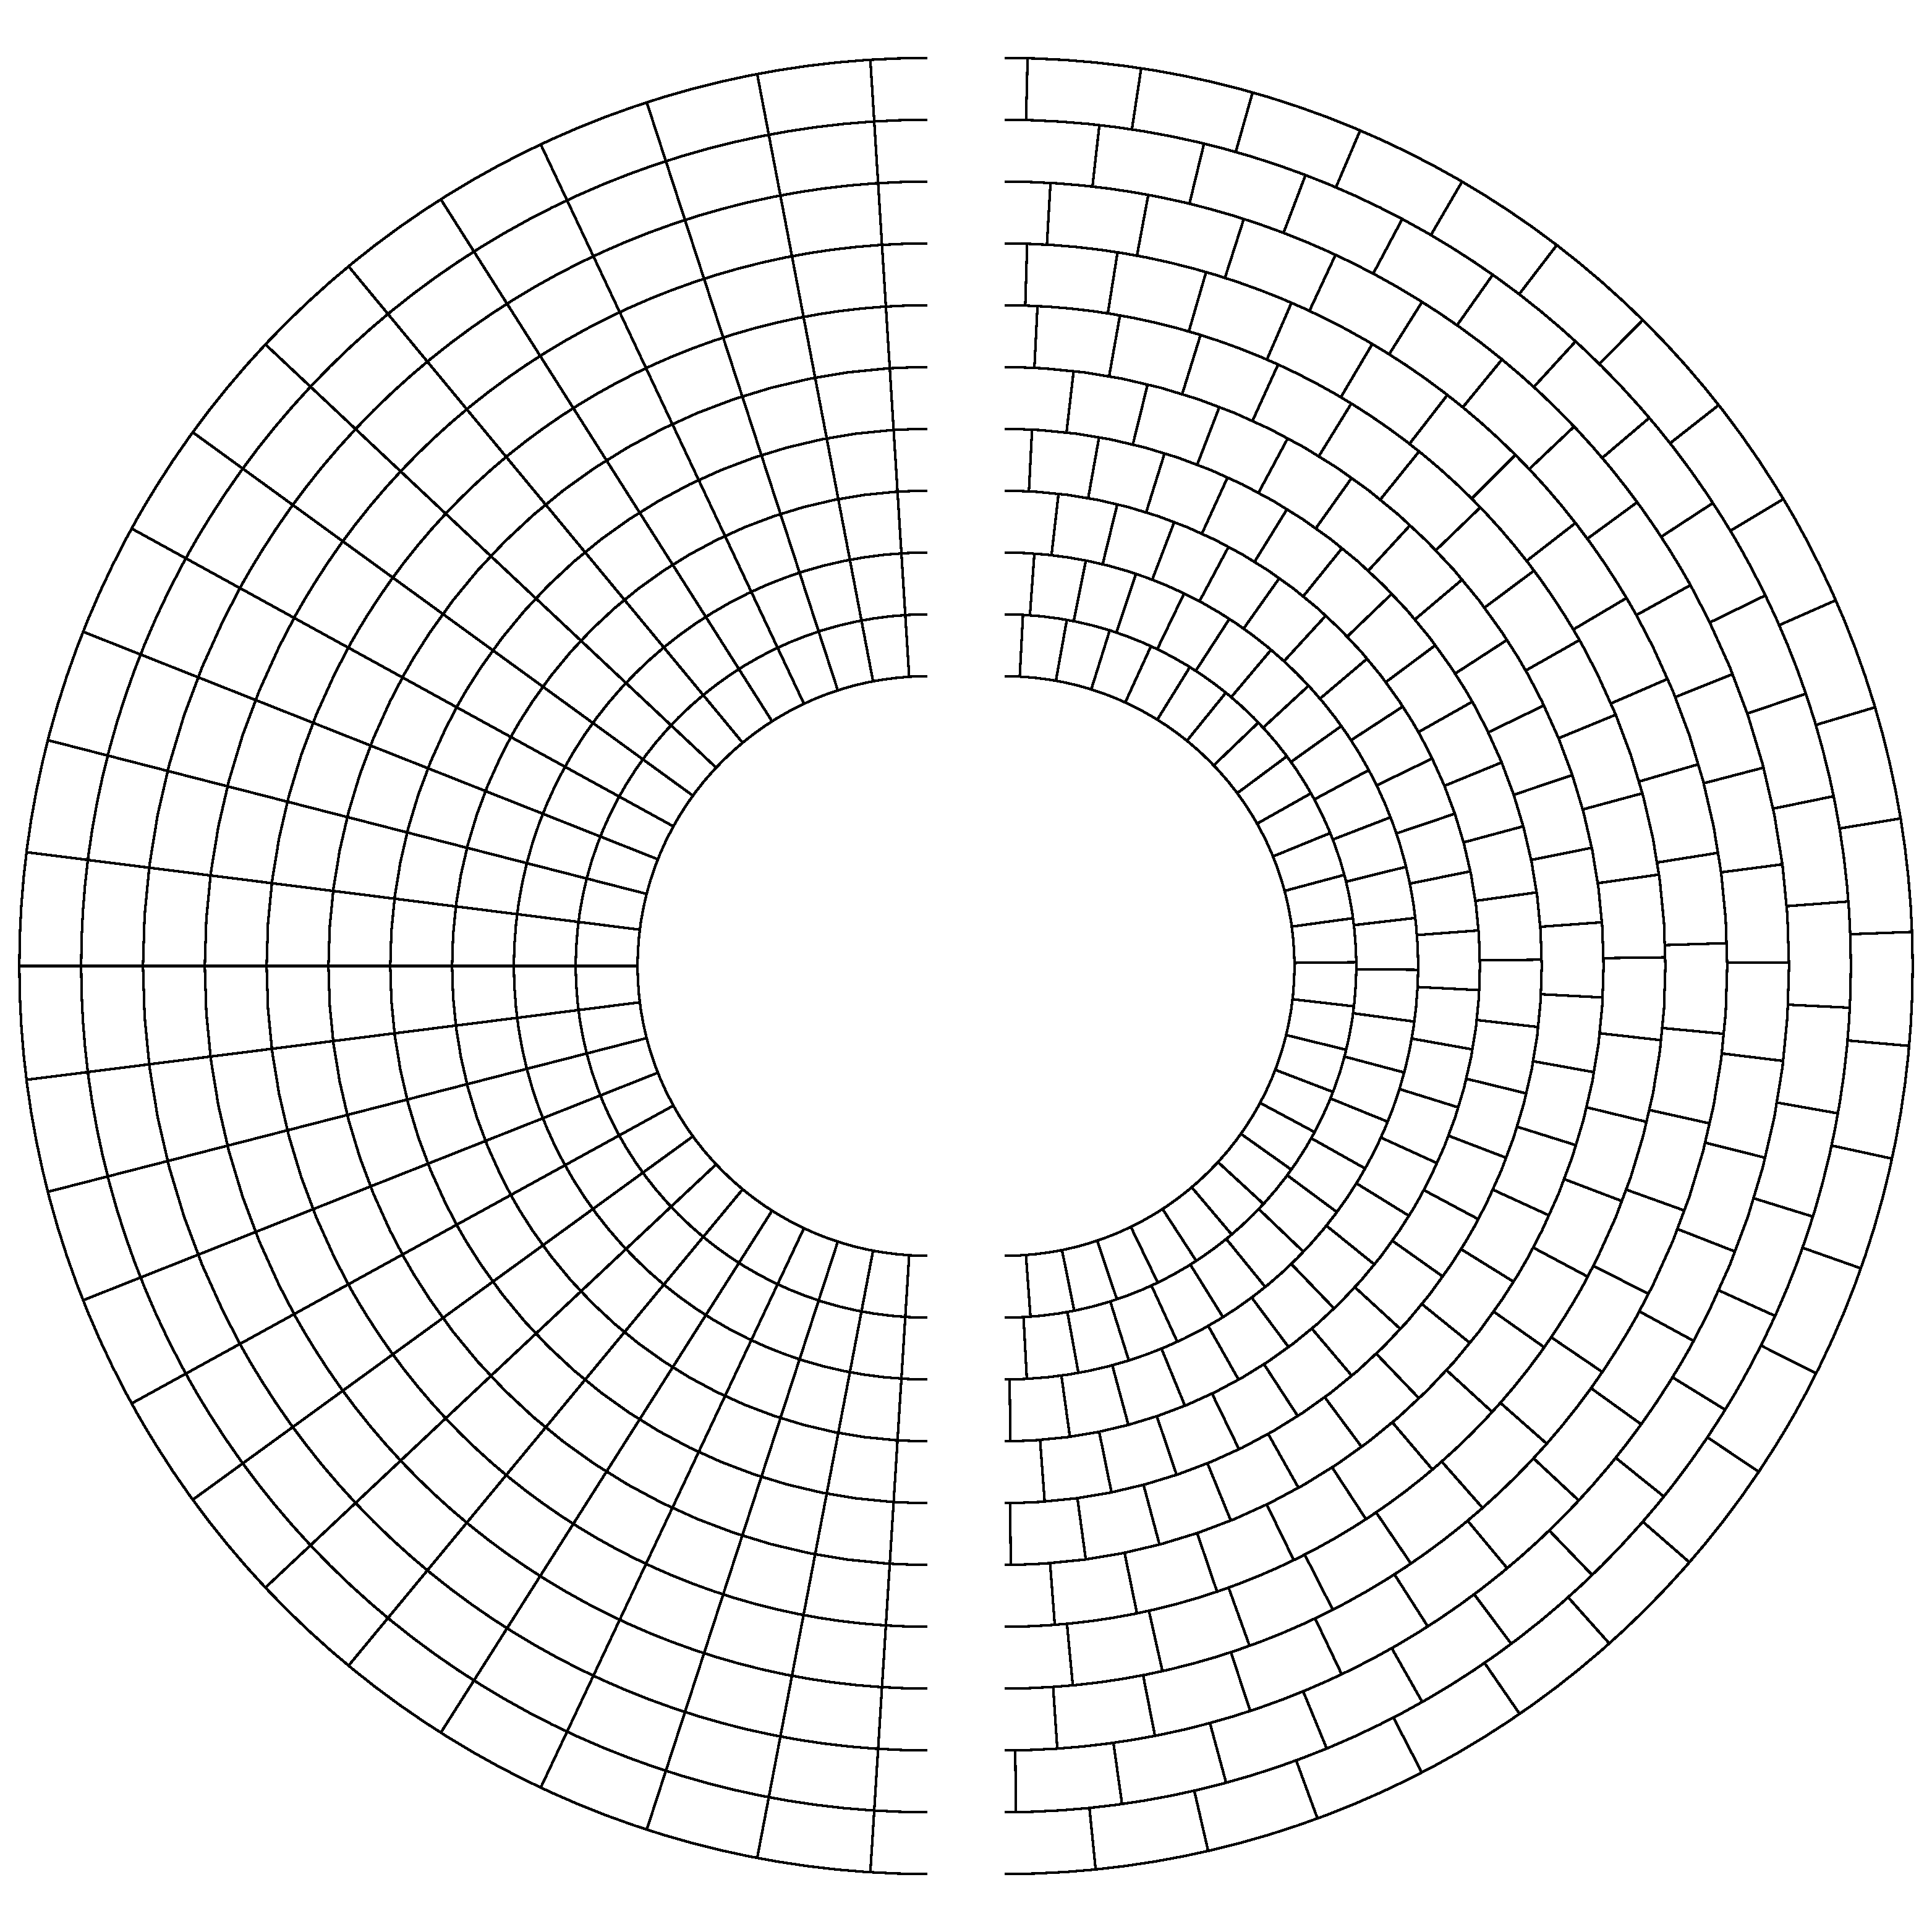
\includegraphics[width=0.6\columnwidth]{img/grid_states.pdf}
\caption{Grid states. Initial grid state (left) and shifted state after some arbitrary number of simulation steps (right).}
\label{fig:grid_states}
\end{figure}

In the original model defined by \ref{eq:ode_1} and \ref{eq:ode_2} \cite{msmm1999}, gravitational acceleration is constant, but in our case, we substitute it by $f_g$, which is assigned individually to each layer of cells, and we refer to this function as \emph{gravity profile}

\begin{equation}
    f_{\text{g}}(i) = \frac{g_i}{g_{\text{out}}},
    \label{eq:gravity_profile_0}
\end{equation}

where $g_{\text{out}}$ is value of gravitational acceleration in the outermost layer $i=0$, and $g_i$ in ${i-\mathrm{layer}}$; in the edge layer its value is ${f_{\text{g}}(i=0) = 1}$, which is the same as in the original MSM. The value of $g_i$ for any layer is 

\begin{equation}
    g_i = \frac{GM_{\text{p}}}{r_i^2},
    \label{eq:gravity_profile_layer}
\end{equation}

where $G$ represents the universal gravitational constant, and $M_{\mathrm{p}}$ is the mass of the primary central object (i.e., the white dwarf). By substituting \eqref{eq:gravity_profile_layer} into \eqref{eq:gravity_profile_0} the $GM_{\text{p}}$ components cancels out, and we get the \emph{gravity profile} function that depends only on layer index $i$

\begin{equation}
	f_{\text{g}}(i) = \left( \frac{r_{\text{out}}}{r_i} \right)^2.
	\label{eq:gravity_profile_final}
\end{equation}

Similarly to the \emph{gravity profile}, we need to tackle the differences in angular velocities between layers to be able to rotate the layers properly. Simply put, if the outer layer moves by one angular cell length in one step, then any subsequent layer moves by some more. We refer to this relation $f_{\omega}$ as \emph{angular velocity profile}

\begin{equation}
    f_{\omega}(i) = \frac{\omega_i}{\omega_\text{out}},
    \label{eq:av_profile_0}
\end{equation}

where $\omega_{\text{out}}$ is angular velocity in the outer layer and $\omega_i$ in arbitrary layer. Angular velocity in the specific layer is

\begin{equation}
    \omega_i = \frac{v_i}{r_i},
    \label{eq:omega_layer}
\end{equation}

where $v_i$ is the orbital velocity

\begin{equation}
    v_i^2 = \frac{G M_{\text{p}}}{r_i}.
    \label{eq:velocity_layer}
\end{equation}

Substituting \eqref{eq:velocity_layer} into \eqref{eq:omega_layer} and than into \eqref{eq:av_profile_0} yields the final form of \emph{angular velocity profile}

\begin{equation}
	f_{\omega}(i) = \left(\frac{r_{\text{out}}}{r_i}\right)^{3/2}.
\end{equation}

Angular position of any cell is expressed by its azimuth $\theta$, and knowing the function $f_{\omega}(i)$, we can get the angular change in one step $\Delta \theta$ for any layer

\begin{equation}
	\Delta \theta (i) = f_{\omega} \frac{2 \pi}{J},
	\label{eq:delta_azimuth} 
\end{equation}

and this expression fully defines the rotational shift for any cell during one simulation step.

Lastly, in our modification, $Q$ depends on the specific behavior of neighboring cells, unlike the original value defined by \eqref{eq:ode_2}. Each cell essentially contains its \emph{leaky faucet}, taking the mass from other cells and redistributing it further into lower cells upon reaching the critical condition. This critical condition is the same as the original MSM

\begin{equation}
	z_c = 5.5.
	\label{eq:z_critical_model}
\end{equation}

\subsection{Modeled system geometry}

To demonstrate our model on a particular case, we consider our modeled system to be a typical \emph{cataclysmic variable star}. The primary component would be a \emph{white dwarf}, whose mass $M_{\text{p}}$ can range from $0.15 M_{\odot}$ up to $1.44 M_{\odot}$. The heaviest observed white dwarf has a mass of $1.35 M_{\odot}$ \cite{caiazzo2021}, so we can limit ourselves to this number instead.

We set the inner disk radius $r_{\text{in}}$ equal to the white dwarf radius. According to \cite{shapiro1983}, the white dwarf \emph{mass to radius ratio} is used to get its approximate radius

\begin{equation}
    r_{\text{in}} \sim M_{\text{p}}^{-1/3}.
\end{equation}

The primary component's Roche lobe constrains the accretion disk, and the outer radius $r_{\text{out}}$ represents the disc's outer edge. For simplicity, we consider the orbits circular, and the $r_{\text{out}}$ is set to correspond with Lagrangian point $L_1$ and is calculated by

\begin{equation}
    r_{\text{out}} = d \left[ \frac{M_{\text{s}}}{3 (M_{\text{p}}+M_{\text{s}})} \right]^{1/3},
\end{equation}

where $d$ represents distance between components of our binary system and $M_{\text{s}}$ is the mass of the secondary donor star. The secondary star is a red giant, massing from $0.3M_{\odot}$ to $8M_{\odot}$. 

\subsection{Optimal grid dimensions}

Knowing the disc boundaries, we then discretize the space in between into regular intervals. Therefore the only other parameter that determines the layer-specific radius $r_i$ for any layer is the $I$ dimension

\begin{equation}
    r_i = r_{\text{in}} + \frac{r_{\text{out}} - r_{\text{in}}}{I - 1} (I - i - 1).
\end{equation}

Considering the orbits are circular, and there is no gravitational interaction between parts of the disc, the orbital period of a particle on Keplerian orbit is determined only by the central mass and radius of the orbital trajectory. Therefore, an implementation assumption of MDH is that the outermost layer moves by exactly one \emph{angular cell length} in one simulation step $\Delta t$. It means that the number of cells in one layer (i.e., the $J$ dimension) and the central object parameters give us the shortest flickering time interval that the simulation can produce.

The main goal of our MDH model is to create a synthetic flickering light curve with a time scale of variability similar to real-world data. Observations show that we need to push this limiting time $\Delta t$ to at least the order minutes, or better seconds. To get the actual relation between dimension $J$ and the minimal time $\Delta t$, we first need to get the orbital period $\tau$ for the layer $i=0$

\begin{equation}
    \tau_{0} = \sqrt{\frac{4 \pi^2 r_{\text{out}}^3}{G M_{\text{p}}}},
    \label{eq:outer_layer_tau}
\end{equation}

where $G$ is the gravitational constant. The $J$ dimension then is

\begin{equation}
	J = \frac{\tau_{0}}{\Delta t}.
	\label{eq:j_dimension}
\end{equation}

Rounding the result of \eqref{eq:j_dimension} to integer gives us the $J$ dimension for chosen time $\Delta t$. We could also use this relation the other way around, choose the dimension first, and then see what time scale this arrangement will give. The downside of this approach is that the shorter the time $\Delta t$ is, the larger the $J$ dimension gets; therefore, the simulation will be more computationally demanding.

The other dimension $I$ can either be a fixed number or be related to the dimension $J$. For this study, we chose a relation that creates somewhat spatially consistent cells in the simulation grid

\begin{equation}
	I = \frac{J}{2 \pi}.
	\label{eq:i_dimension} 
\end{equation}

Again, rounding the result of \eqref{eq:i_dimension} integer. It is self-evident that the grid size can quickly get upwards of tens of thousands of individual simulation cells. Therefore great emphasis needs to be placed on parallelization and code optimization. 

\subsection{The cellular automaton algorithm}

Actions performed during one simulation step are divided into a series of simple operations that include cell orbital movement, matter redistribution, and temperature changes. The basic algorithmic structure of MDH is

\begin{enumerate}
	\item Rotate all the layers according to \eqref{eq:delta_azimuth}.
	\item Find the cell closest to chosen value of $\theta$ (typically $\theta = 0$) in the outermost layer $i = 0$, and add the $q$ amount of matter to it; see \eqref{eq:q_estimate}.
	\item Solve the ODE system \eqref{eq:ode_1} and \eqref{eq:ode_2} for all cells using an iterative method out of the Runge-Kutta family; in our case, the Runge-Kutta-Fehlberg (RKF78).
	\item If any cell reaches the critical condition \eqref{eq:z_critical_model}, the mass outflow is triggered in that cell.
    \item Calculate temperature changes for all cells according to the processes described in Section \ref{sec:thermal_processes}.
	\item Save all cell states and repeat the process for the next step.
\end{enumerate}

The MSM's mass scale differs from the global mass scale of the whole accretion disk. However, it is not a problem because we are using the MSM only as the chosen critical condition, and we are primarily interested in its qualitative rather than quantitative properties. Still, we need to know the disc's global amount of transferred mass.

For a typical CV binary system, we assume the accretion rate \cite{ae_shortrev2015}

\begin{equation}
	\dot{M} \sim 10^{14}\, \mathrm{g \cdot s^{-1}},
\end{equation}

and as shown in \cite{msmm1999} the value of $q$ is

\begin{equation}
	\label{eq:q_estimate}
	q \sim 10^{-1}\, \mathrm{g},
\end{equation} 

therefore, we can propose a relation between the accretion rate $\dot{M}$ and the internal value of $q$

\begin{equation}
	q \propto \dot{M} \cdot \Delta t.
\end{equation}

The mass added to the disk in sub-step 2 of the algorithm would fill up only the outer layer. Other subsequent layers get their mass from the cell above when they reach the critical condition \eqref{eq:z_critical_model}.

At the moment of \emph{dripping}, part of the mass breaks from the source cell and moves into lower adjacent cells. The amount of mass $\Delta m$ that breaks out of the cell is

\begin{equation}
	\Delta m = \psi \cdot m_{ij}
	\label{eq:delta_m}
\end{equation}

where the exact value of $\psi \in [0;1]$ serve as another free parameter in the simulation. We computed the presented Results using $\psi = 0.8$. To keep the simulation numerically stable, it is also necessary to introduce a low-value cut-off for the cell's mass $m_{ij}$. We use the following relation to determine the cell's mass after the breakout    

\begin{equation}
    \begin{aligned}
        & m_{ij}~= 
        \begin{cases}
            m_{ij} - \Delta m \hspace{5mm} (m_{ij} \ge 10^{-8}) \\
            \hspace{8mm} 0 \hspace{12mm} (m_{ij} < 10^{-8}).
        \end{cases}
    \end{aligned}
    \label{eq:m_cut_off}
\end{equation}

The amount of mass $\Delta m$ transfers into lower adjacent cells. There are always no more than two lower layer cells in contact with the source cell, as evident from Figure \ref{fig:grid_states}; therefore, the redistribution algorithm finds the two closest cells and splits the mass $\Delta m$ between the two receiving cells. The mass split is directly proportional to the relative length of contact the adjacent cells have with the source cell.   


% \section{Cell definition}
% Individual cells are defined by a set of parameters. These parameters are listed in table \ref{table:mdh_cell_parameters}, and the following sections discuss some of them in detail.
%
% \begin{table}[h]
% \begin{center}
% \begin{tabular}{r|l}
% $i$			& Layer index \\
% $j$			& Cell index \\
% $r$			& Orbital radius \\
% $\theta$	& Orbital azimuth \\
% $f_g$		& Gravitational acceleration relative to outermost layer \\
% $z$			& MSMM \emph{spring elongation}  \\
% $v$			& MSMM \emph{velocity} \\
% $m$			& Mass contained within the cell \\
% $\Delta m$ 	& Mass change since previous step \\
% $\gamma$		& Constant MSMM dampening parameter \\
% $k$			& MSMM \emph{spring stiffness} \\
% $T$			& Cell temperature
% \end{tabular}
% \caption{MDH model cell parameters}
% \label{table:mdh_cell_parameters}
% \end{center}
% \end{table}
%
% \begin{figure}[H]
% \centering
% 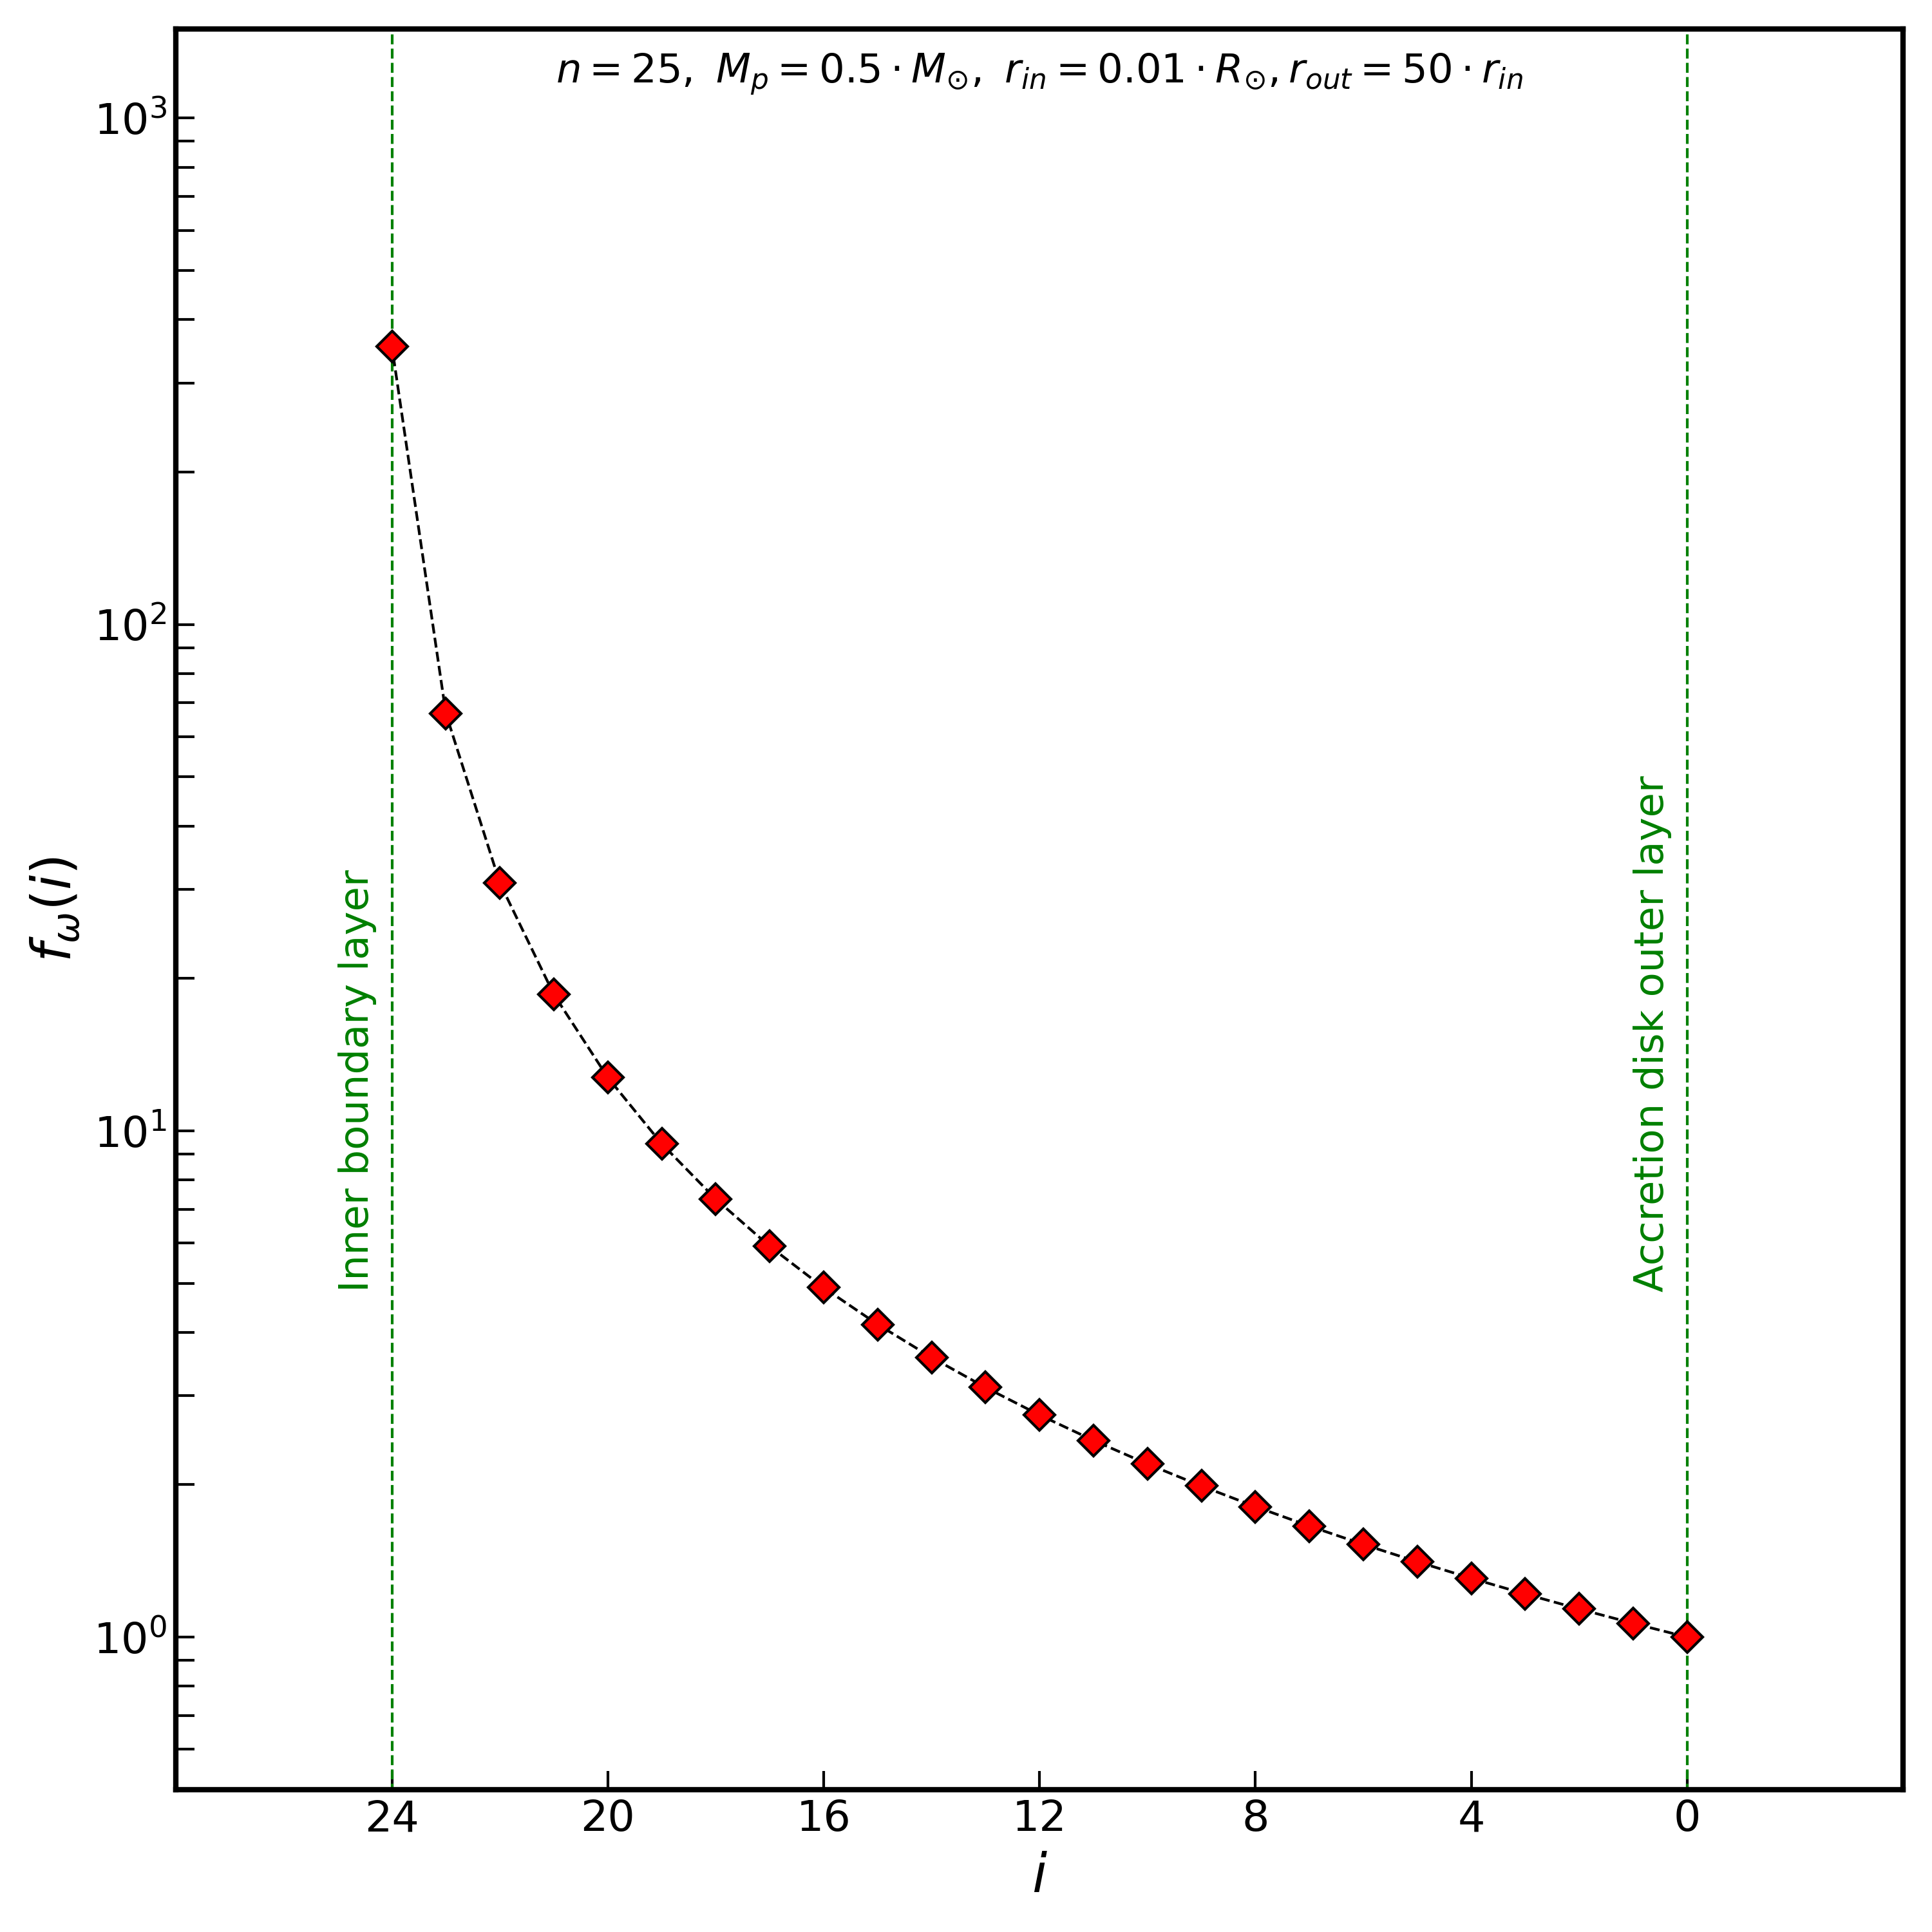
\includegraphics[width=0.9\columnwidth]{img/profile_omega.png}
% \caption{Angular velocity profile relative to the layer $i = 0$ with modelled system parameters: $n=25$, $M_p = 0.5 \cdot M_{\odot}$, $r_{in} = 0.01 \cdot R_{\odot}$, $r_{out} = 50 \cdot r_{in}$}
% \label{fig:profile_omega}
% \end{figure}
%
% \begin{figure}[H]
% \centering
% 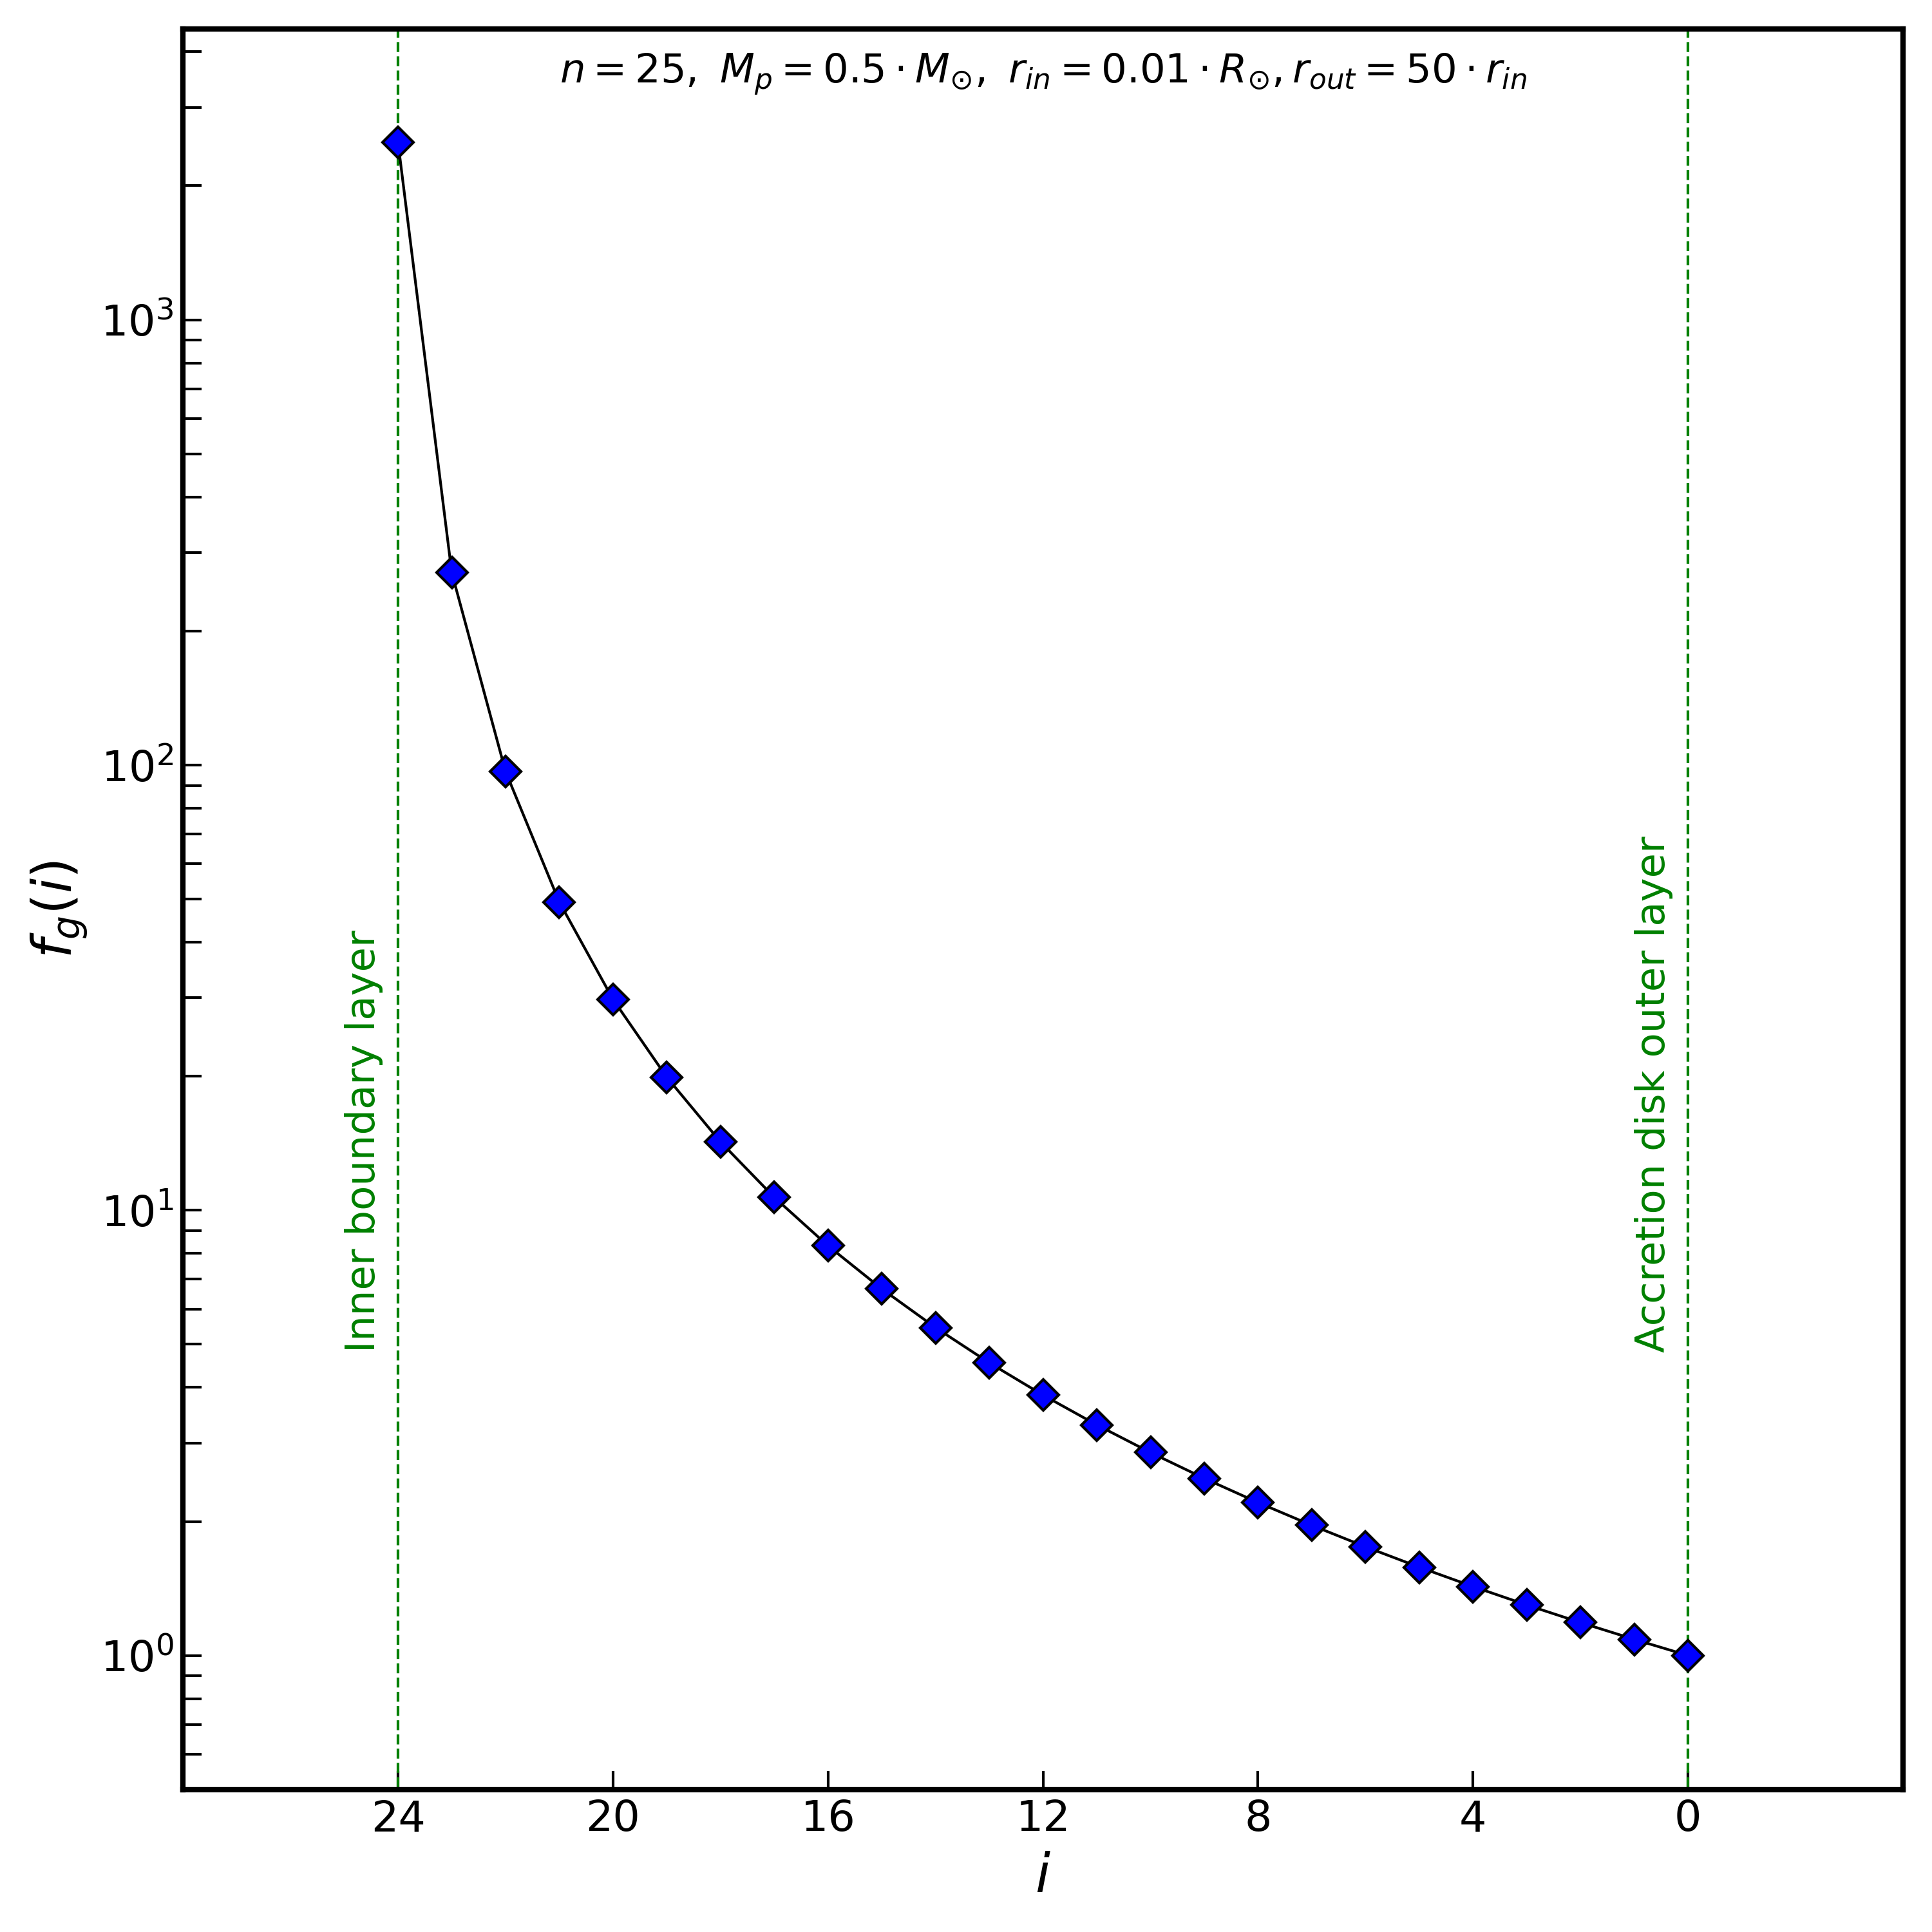
\includegraphics[width=0.9\columnwidth]{img/profile_g.png}
% \caption{Gravity profile relative to the layer $i = 0$ with modelled system parameters: $n=25$, $M_p = 0.5 \cdot M_{\odot}$, $r_{in} = 0.01 \cdot R_{\odot}$, $r_{out} = 50 \cdot r_{in}$}
% \label{fig:profile_g}
% \end{figure}
%


%%%%%%%%%%%%%%%%%%%%%
% Thermal processes %
%%%%%%%%%%%%%%%%%%%%%

\section{Thermal processes}
\label{sec:thermal_processes}

The principal observational quantity is a light curve, which derives from the radiation properties of our model, mainly the temperature. To extract light curves out of our dynamical matter flow simulation, we need to know the temperature of every cell at any given moment throughout the simulation. We apply the black-body approximation, and to simplify the situation, we assume the cells to be optically thin. 

Every cell's temperature is a value undergoing continuous change; it depends on the temperature in previous simulation steps and not solely on external parameters.

The essential factor for consequent thermal processes is the temperature of the matter that flows into the disk from the outside. Its value is determined mainly by the given properties of the secondary star, and in the case of the late-type star, according to \cite{allen1973}, we expect it to be

\begin{equation}
T_{\text{out}} \sim 10^3\, \mathrm{K}.
\end{equation}

We can establish three main mechanisms of temperature change and will discuss them more closely below. A summary of those will yield the final temperature. 

\subsection{Free-Free emission heating}

At the moment of \emph{dripping}, the matter that falls into a lower layer cell losses some potential energy \cite{yonehara1997} 

\begin{equation}
   \Delta E_{ij} = \frac{1}{2} G M_{\text{p}} \Delta r \frac{\Delta m_{ij}}{r_i^2},
   \label{eq:e_pot}
\end{equation}

where $\Delta m_{ij}$ represents the falling mass and $\Delta r$ the layer width, i.e., the distance traveled by the mass. 

This energy is released by the process of \emph{free-free emission} (i.e. bremsstrahlung); with some efficiency $\varepsilon$ is transformed into internal energy $U$ of the receiving cell

\begin{equation}
	\Delta U_{i+1,j} = \varepsilon \Delta E_{ij},
\end{equation}

where $\Delta U_{i+1,j}$ represents the change of receiving cell's internal energy that heats up the cell. For the sake of simplicity, the heating efficiency is considered to be ${\varepsilon=1}$, then  

\begin{equation}
	\Delta U_{i+1,j} \equiv \Delta E_{ij}.
	\label{eq:e_int_pot_equiv}
\end{equation} 

Gas internal energy change is related to the temperature change by

\begin{equation}
	\Delta U_{ij} = \frac{3}{2} n_{ij} \mathcal{R} \Delta T_{ij},
	\label{eq:e_int_temp_relation}
\end{equation}

where $\mathcal{R}$ is the ideal gas constant, and $n_{ij}$ is the number of moles of gas within the cell. Because it is considered to be mostly hydrogen, and its molar mass is $M_{\text{H}} \approx 1$, we can use mass $m_{ij}$ and the number of moles $n_{ij}$ interchangeably. By substituting \eqref{eq:e_int_temp_relation} and \eqref{eq:e_pot} into \eqref{eq:e_int_pot_equiv}, and rearranging a bit, we get the expression that relates change of cell's temperature in layer $i+1$, to the amount of mass falling from the cell above

\begin{equation}
	\Delta T_{i+1,j} = \frac{1}{3} \frac{G M_{\text{p}} \Delta m_{ij} \Delta r}{r_{i}^2 \mathcal{R} m_{i+1,j}}.
	\label{eq:temp_ff_final}
\end{equation}

\subsection{Gas mixing}

Another mechanism we need to consider is mixing different temperatures and amounts of gases when the dripping occurs. We need to describe the temperature change for the donor cell $T_{ij}$ and the receiving $T_{i+1,j}$. Both instances can be solved utilizing changes in the cell's internal energy, and on the donor side, the resulting expression is simply  

\begin{equation}
T_{ij}' = T_{ij},
\end{equation}

where $T_{ij}$ and $T_{ij}'$ are the temperatures before and after the mass outflow, respectively. In the case of the receiving cell, we are mixing two different amounts of gas at two different temperatures, and the expression is

\begin{equation}
T_{i+1,j}' = \frac{m_{i+1,j} T_{i+1,j} + \Delta m_{ij} T_{ij}}{m_{i+1,j} + \Delta m_{ij}}.
\end{equation}

\section{Radiative cooling}

The third mechanism influencing the cell temperature is radiative cooling. We use an approximation that the cells of an optically thin disk radiate as black-body through their top and bottom facets, and one facet having the area

\begin{equation}
	S_{ij} = \frac{2 \pi r_i \Delta r}{J},
	\label{eq:facet_area}
\end{equation}

where $\Delta r$ represents the layer width. Conversion of the cell's internal energy in relation to its black-body radiation is

\begin{equation}
	\frac{3}{2} m_{ij} \mathcal{R} \frac{dT_{ij}}{dt} = \sigma T_{ij}^4 S_{ij},
	\label{eq:rad_cooling_temp_0}
\end{equation}

where $\sigma$ is the Stefan-Boltzman constant. Integrating the \eqref{eq:rad_cooling_temp_0} and rearranging a bit yields the expression for the cell's temperature, which is in the local thermodynamic equilibrium of the radiative cooling

\begin{equation}
T_{ij}' = \left( \frac{2 \sigma S_{ij} t}{m_{ij} \mathcal{R}} + \frac{1}{T_{ij}^3} \right)^{-1/3}.
\end{equation}

%%%%%%%%%%%%%%%%%%%%%%%%%%%%%%%%%%%%
% Synthetic light curve extraction %
%%%%%%%%%%%%%%%%%%%%%%%%%%%%%%%%%%%%

\section{Synthetic light curves}

Knowing the temperatures of all cells throughout the simulation, as a result of thermal processes define in Section \ref{sec:thermal_processes}, enables us to extract simulated spectra. Cell's radiation power at a specific wavelength from both top and bottom facets is given by

\begin{equation}
	L_{\lambda,ij} = 4\pi \cdot S_{ij} \cdot B_{\lambda,ij}(\lambda, T_{ij}),
	\label{eq:facet_radiation}
\end{equation}

where $B_{\lambda}(\lambda, T_{i,j})$ represents flux density in the given point by the Planck's function, $S_{ij}$ is a single radiating facet area defined by \eqref{eq:facet_area}. Because the accretion disk is considered optically thick, the single facet radiates into the solid angle of $2\pi$. 

% Figure \ref{fig:spectum_comparison} shows spectra extracted from two distinct simulation runs, one of which (red) was disturbed by a blob of mass impacting the accretion disk (see text (a) and (b) in section 5). Both spectral curves come from the same point in their respective runs (step 1050), which is shortly after the impact for the disturbed run.

% \begin{figure}[ht]
	% \centering
	% 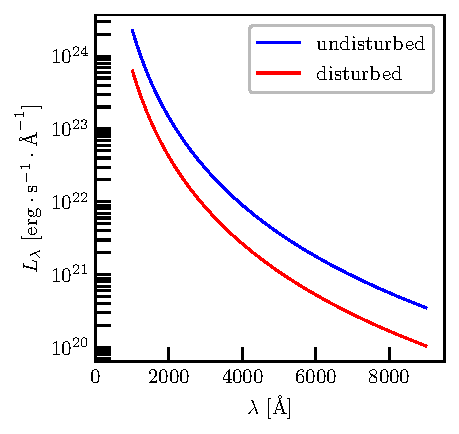
\includegraphics{img/spec_d1050_d1050.pdf}
	% \caption{Comparison of two spectral curves extracted from undisturbed stabilized run (blue) and blob disturbed (red) run.}
	% \label{fig:spectum_comparison}
% \end{figure}
%
% It is evident from Figure \ref{fig:spectum_comparison} that the temperature increase caused by the impacting mass shifts slightly the peak of radiation towards shorter wavelengths, and thus effectively lowers the total radiation power in the wavelength of our interest (i.e., roughly the range covered by $\mathcal{UBVRI}$ system).

\subsection{Light curves in a photometric filter}

To simulate observational data more closely, we apply an analytic approximation of Johnson-Cousins $\mathcal{UBVRI}$ filters onto the wavelength-specific total power output of the disk, and we get the synthetic light curve for the chosen filter. The approximation is expressed by

\begin{equation}
g(\lambda) \propto \text{exp}\left[ - \frac{1}{2} \left( \frac{\lambda - \lambda_{\text{c}}}{\lambda_{\mathrm{w}}} \right)^2 \right],
\label{eq:filter_gauss}
\end{equation}

where $\lambda_{\mathrm{c}}$ specifies the effective central wavelength of the specific filter, and $\lambda_{\mathrm{w}}$ is the effective filter width. Johnson-Cousins specific approximative values are shown in Table 1.

\begin{table}[ht]
\centering
\begin{tabular*}{\columnwidth}{@{\extracolsep{\fill}}ccc}
Filter & $\lambda_{\mathrm{c}}$ $[\text{\r{A}}]$ & $ \lambda_{\mathrm{w}}$ $[\text{\r{A}}]$\\
\hline\hline
$\mathcal{U}$ & 3663 & 650\\
$\mathcal{B}$ & 4361 & 890\\
$\mathcal{V}$ & 5448 & 840\\
$\mathcal{R}$ & 6407 & 1580\\
$\mathcal{I}$ & 7980 & 1540\\
\hline
\end{tabular*}
\caption{Parameters of Johnson-Cousins $\mathcal{UBVRI}$ filters approximation. \cite{bessell2005}}
\end{table}

The radiation power is computed for every cell step by step. Using \eqref{eq:facet_radiation} and \eqref{eq:filter_gauss} and summing up all the cells, we get filtered power output $L_{\mathrm{F}}$ from both sides of the accretion disk

\begin{equation}
L_{\mathrm{F}} = 4 \pi S_{ij} \Delta \lambda \sum_{i=0}^{I-1} \sum_{j=0}^{J-1} \sum_{\lambda=0}^{\infty} B_{\lambda,ij}(\lambda, T_{ij})\,g(\lambda),
\end{equation}

where $\Delta \lambda$ represents wavelength integration step.

